For the literature review, mathematical detail was kept to a minimum for clarity of presentation. In this chapter we revisit some basics of inference and particle filtering in order to establish notation and mathematical foundations for the later chapters.

Many tasks in signal processing, science in general, and indeed life, require us to make some estimate of an unknown quantity from indirect, incomplete, or inaccurate observations. By constructing a probabilistic model to explain how these observations depend on the underlying state, we can infer something about that state. Such an observation model may be expressed in terms of a likelihood function:

\begin{equation}
P(Y|X)
\label{eq:LH}
\end{equation}

where $X$ is the state and $Y$ the observations. This is not the whole story - in many cases we are not estimating our unknown state `from scratch'. Previous experience, prejudice, and prior knowledge can also contribute to our estimates. The likelihood and prior terms can be combined through our friend, Bayes rule \cite{Bayes1763,Laplace1774}, to calculate the posterior probability of the state, i.e. the probability of the state given the observations:

\begin{equation}
P(X|Y) = \frac{P(Y|X)P(X)}{P(Y)}
\label{eq:BayesRule}
\end{equation}

This is the basis of the process of inference. Mathematically, we can assign a probability distribution to the state space of $X$. By applying Bayes rule, we are updating our belief about the values of $X$ using the information in $Y$.

Often the quantity in which we are interested, $X$, is changing over time, and it is desirable to estimate its value at each point in time given only the observations received so far. In this case, a hidden Markov model may be employed for the state evolution process, shown graphically in figure~\ref{fig:HMM}. This is the traditional filtering problem. %The Markovian assumption, that $X_t$ is independent of $X_{1:t-2}$ when conditioned on $X_{t-1}$, can generally be justified by a suitable choice of variables in $X_t$.

\begin{figure}[hbt]%
\centering

\tikzstyle{state} = [circle,thick,minimum size=1.2cm,draw=black]
\tikzstyle{assoc} = [circle,thick,minimum size=1.2cm,draw=blue]
\tikzstyle{observ} = [circle,thick,minimum size=1.2cm,draw=red]

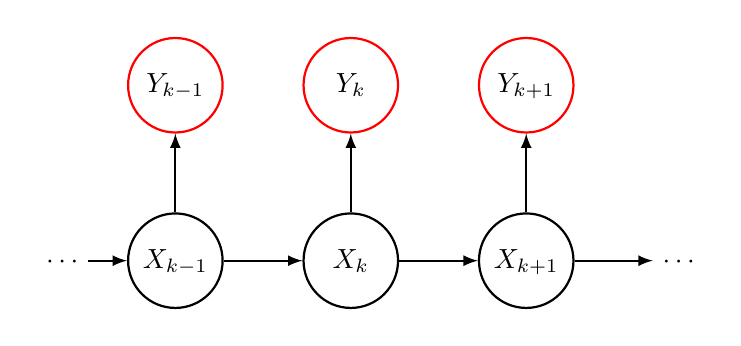
\begin{tikzpicture}[>=latex,text height=1.5ex,text depth=0.25ex]

	\matrix[row sep=0.5cm,column sep=0.5cm] {
		&
		\node (y_k-1) [observ]{$Y_{k-1}$}; &
		&
		\node (y_k) [observ]{$Y_{k}$}; &
		&
		\node (y_k+1) [observ]{$Y_{k+1}$}; &
		& \\
		& & & & & & & \\
		\node (x_k-2) {$\cdots$}; &
		\node (x_k-1) [state]{$X_{k-1}$}; &
		&
		\node (x_k) [state]{$X_{k}$}; &
		&
		\node (x_k+1) [state]{$X_{k+1}$}; &
		&
		\node (x_k+2) {$\cdots$}; \\
	};

	\path[->]
		(x_k-2) edge[thick] (x_k-1)
		(x_k-1) edge[thick] (x_k)
		(x_k) edge[thick] (x_k+1)
		(x_k+1) edge[thick] (x_k+2)
		
		(x_k-1) edge[thick] (y_k-1)
		(x_k) edge[thick] (y_k)
		(x_k+1) edge[thick] (y_k+1)
		;

\end{tikzpicture}
\caption{Graphical hidden Markov model.}%
\label{fig:HMM}%
\end{figure}

Our prior information about the state can now be derived from the estimate of its value at the previous time step with a forward prediction operation.

\begin{equation}
P(X_t|Y_{1:t}) = \frac{\int P(Y_t|X_t)P(X_t|X_{t-1})P(X_{t-1}|Y_{1:t-1}) dX_{t-1}}{P(Y_t|Y_{1:t-1})}
\label{eq:SeqBayesRule}
\end{equation}

where the subscript indicates the time and ranges are notated by $:$ in the MATLAB style. $P(X_t|Y_{1:t})$ is called the filtering distribution. Equation~\ref{eq:SeqBayesRule} describes the ideal Bayesian filter.

%Instead of marginalising the previous state, we may sometimes want to consider the joint state distribution over all time instances. This may similarly be expanded as:

%\begin{equation}
%P(X_{1:t}|Y_{1:t}) = \frac{P(Y_t|X_t)P(X_t|X_{t-1})P(X_{1:t-1}|Y_{1:t-1})}{P(Y_t|Y_{1:t-1})}
%\label{eq:JointSeqBayesRule}
%\end{equation}

%The filtering distribution may then be obtained by marginalising out the previous states.

%So far, we have expressed the problem entirely in terms of distributions. The same models may be expressed in terms of difference equations of random variables. In the most general form:
%\begin{equation}
%X_t = f_t(X_{t-1}, V_t)
%\label{eq:FilterEq1}
%\end{equation}
%\begin{equation}
%Y_t = g_t(X_t, W_t)
%\label{eq:FilterEq2}
%\end{equation}

%where $f_t$ and $g_t$ are known deterministic functions and $V_t$ and $W_t$ and random variables, known as the process and observation noise respectively.
